% Required packages: amsmath, amssymb, xcolor, tikz
% Required TikZ libraries: none
% Target width: 160 mm
% Minimum text size: 8 pt
% Colour/greyscale intent: one teal accent; grouping and direct labels survive greyscale
% Generated from paper/results/nano-diagnosis.json by analysis/make_diagnosis_figure.py.
\begingroup
\definecolor{ealnanoaccent}{RGB}{15,91,103}
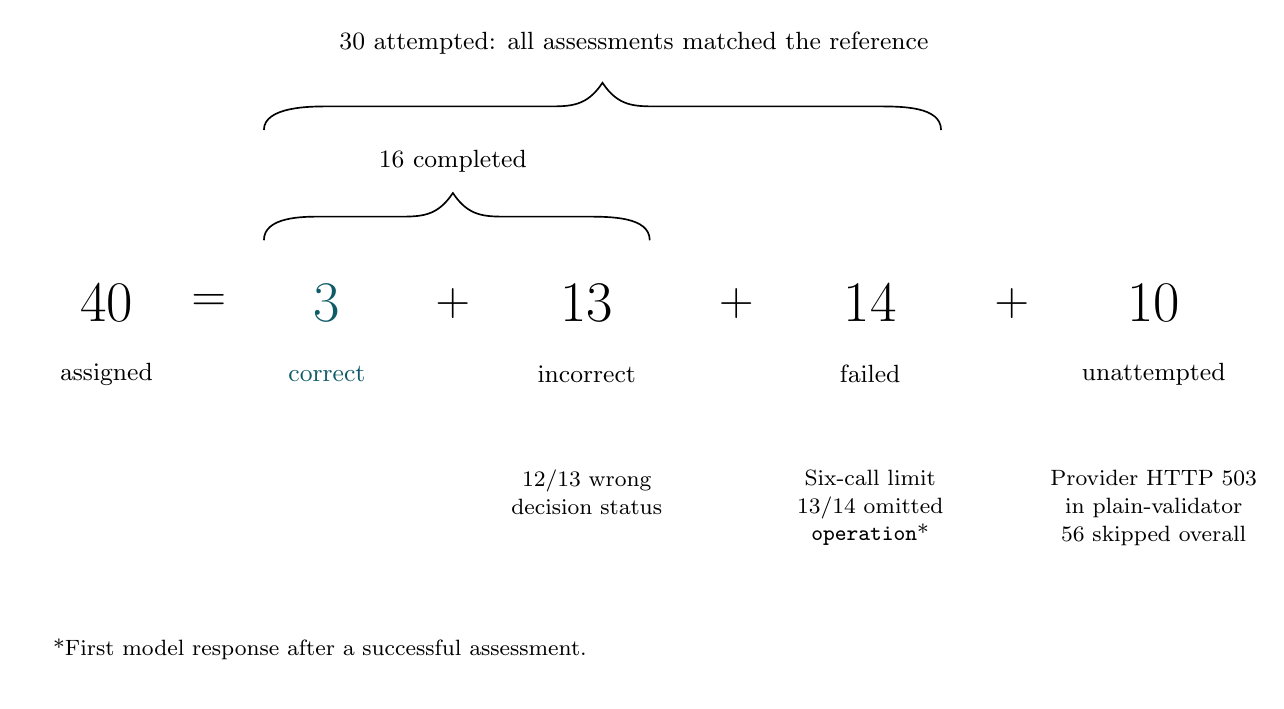
\begin{tikzpicture}[x=1mm,y=1mm,font=\fontsize{9}{11}\selectfont]
\path[use as bounding box] (0,0) rectangle (156,83);
% Mathematical grouping braces; their extent identifies summands, not a time path.
\draw[line width=.6pt] (30,70) .. controls (30,73) and (36,73) .. (38,73)
 -- (66,73) .. controls (69,73) and (71,73) .. (73,76)
 .. controls (75,73) and (77,73) .. (80,73) -- (108,73)
 .. controls (111,73) and (116,73) .. (116,70);
\node at (77,81) {30 attempted: all assessments matched the reference};
\draw[line width=.6pt] (30,56) .. controls (30,59) and (35,59) .. (37,59)
 -- (47,59) .. controls (50,59) and (52,59) .. (54,62)
 .. controls (56,59) and (58,59) .. (61,59) -- (71,59)
 .. controls (74,59) and (79,59) .. (79,56);
\node at (54,66) {16 completed};
\node[font=\fontsize{22}{24}\selectfont] at (10,48) {$40$};
\node[font=\fontsize{18}{20}\selectfont] at (23,48) {$=$};
\node[font=\fontsize{22}{24}\selectfont,text=ealnanoaccent] at (38,48) {$3$};
\node[font=\fontsize{18}{20}\selectfont] at (54,48) {$+$};
\node[font=\fontsize{22}{24}\selectfont] at (71,48) {$13$};
\node[font=\fontsize{18}{20}\selectfont] at (90,48) {$+$};
\node[font=\fontsize{22}{24}\selectfont] at (107,48) {$14$};
\node[font=\fontsize{18}{20}\selectfont] at (125,48) {$+$};
\node[font=\fontsize{22}{24}\selectfont] at (143,48) {$10$};
\node at (10,39) {assigned};
\node[text=ealnanoaccent] at (38,39) {correct};
\node at (71,39) {incorrect};
\node at (107,39) {failed};
\node at (143,39) {unattempted};
\node[align=center,font=\fontsize{8}{10}\selectfont] at (71,24)
  {12/13 wrong\\decision status};
\node[align=center,font=\fontsize{8}{10}\selectfont] at (107,22)
  {Six-call limit\\13/14 omitted\\\texttt{operation}*};
\node[align=center,font=\fontsize{8}{10}\selectfont] at (143,22)
  {Provider HTTP 503\\in plain-validator\\56 skipped overall};
\node[anchor=west,font=\fontsize{8}{10}\selectfont] at (2,4)
  {*First model response after a successful assessment.};
\end{tikzpicture}
\endgroup
